\documentclass[a4paper, 12pt]{article}
\usepackage{fullpage}

\usepackage{mathtext}
\usepackage[russian]{babel}
\usepackage{amssymb,amsmath,commath}
\usepackage{graphicx}

\usepackage[utf8]{inputenc}
%\usepackage{ulem, cancel}

\usepackage{multirow}

\begin{document}

\section{Теория}

\subsection{Статические деревья отказов}

Легче всего поддаются анализу статические деревья отказов с независимыми поддеревьями. Пример такого дерева приведён на рисунке \ref{fig:sft1}.

\begin{figure}[p]
  \centering
  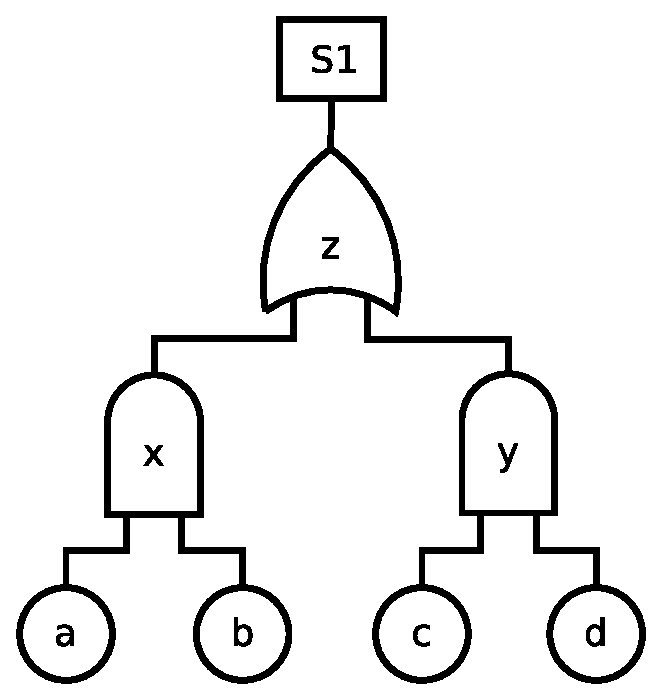
\includegraphics[height=4.0cm]{s1}
  \hspace{1.0cm}
  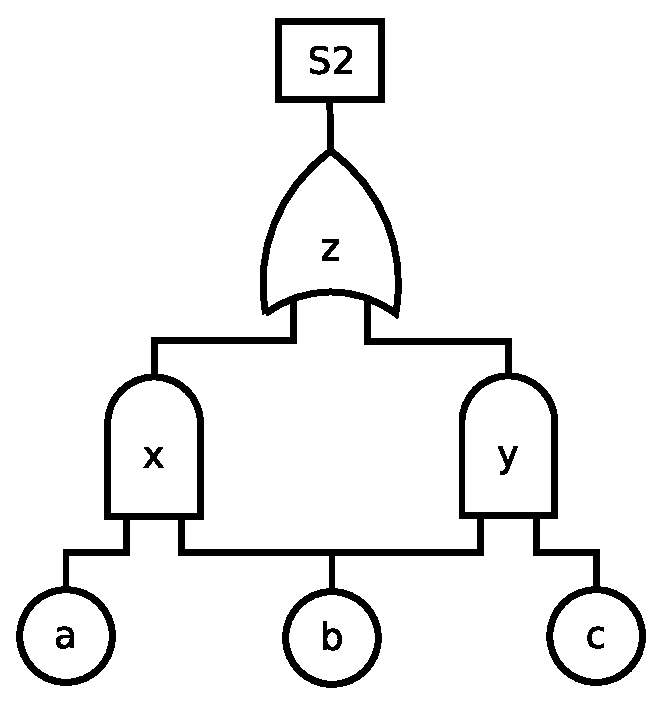
\includegraphics[height=4.0cm]{s2}
  \caption{Два примера статических дерева отказа: с независимыми поддеревьями (слева) и с зависимыми (справа).}
  \label{fig:sft1}
\end{figure}

Круглыми узлами обозначены элементарные события (независимые от остальных). Обычно предполагается, что эти события имеют экспоненциальное распределение, т.е. $P(t_a < t) = F_a(t) = 1 - e^{-\lambda_a t}$, где $P(t_a < t)$ -- вероятность того, что событие $a$ произойдёт до момента $t$ ($F_a(t)$ используется далее по тексту для обозначения распределений величин), $t_a$ -- время события $a$, $\lambda_a$ -- интенсивность события $a$ (задана заранее).

Узлами традиционной формы обозначены логические операции AND и OR. Прямоугольный узел указывает на итоговое событие, которое нужно проанализировать.

Подобные деревья поддаются анализу методами простейшей теории вероятностей. Задавшись интересующим временем $T$, определим вероятности элементарных событий: $p_a = F(T) = 1 - e^{\lambda_a t}$. После этого, используя формулы для вероятностей произведения и суммы событий, получим вероятности всех остальных событий. Для первого дерева на рисунке \ref{fig:sft1} имеем:

\begin{equation*}
  \begin{array}{l}
    p_a = 1 - e^{-\lambda_a T} \\
    p_b = 1 - e^{-\lambda_b T} \\
    p_c = 1 - e^{-\lambda_c T} \\
    p_d = 1 - e^{-\lambda_d T} \\
    p_x = p_a p_b \\
    p_y = p_c p_d \\
    p_z = 1 - (1 - p_x) (1 - p_y) = p_x + p_y - p_x p_y
  \end{array}
\end{equation*}

В случае с зависимыми поддеревьями такой подход неприменим. В таком случае на помощь приходит рассмотрение условных вероятностей и применение правила Байеса. Для комбинирования распределений вводится новое понятие -- условное распределение. Каждый узел AND и OR заменяется соответствующим условным распределением. После этого вся система раскрывается по правилу Байеса и сворачивается по всем переменным, кроме последней, для получения итогового распределения.

\begin{figure}[p]
  \centering
  \begin{tabular}{c|c|c|c|c|}
    \cline{2-5}
    \multirow{2}{*}{$\textrm{AND}_{x|ab}$} & \multicolumn{2}{|c|}{a = 0} & \multicolumn{2}{|c|}{a = 1} \\
    \cline{2-5}
    & b = 0 & b = 1 & b = 0 & b = 1 \\
    \cline{1-5}
    \multicolumn{1}{|c|}{x = 0} & 1 & 1 & 1 & 0 \\
    \cline{1-5}
    \multicolumn{1}{|c|}{x = 1} & 0 & 0 & 0 & 1 \\
    \cline{1-5}
  \end{tabular}
  \begin{tabular}{c|c|c|c|c|}
    \cline{2-5}
    \multirow{2}{*}{$\textrm{OR}_{z|xy}$} & \multicolumn{2}{|c|}{x = 0} & \multicolumn{2}{|c|}{x = 1} \\
    \cline{2-5}
    & y = 0 & y = 1 & y = 0 & y = 1 \\
    \cline{1-5}
    \multicolumn{1}{|c|}{z = 0} & 1 & 0 & 0 & 0 \\
    \cline{1-5}
    \multicolumn{1}{|c|}{z = 1} & 0 & 1 & 1 & 1 \\
    \cline{1-5}
  \end{tabular}
  
  \caption{Условные распределения для узлов AND и OR.}
  \label{fig:sft2}
\end{figure}

Например, для второй системы из рисунка \ref{fig:sft1} распределения элементарных событий и условные распределения событий составных выглядят следующим образом (таблицы распределений AND и OR показаны на рисунке \ref{fig:sft2}):

\begin{equation*}
  \begin{array}{l}
    p_a: \; p_{a=0} = e^{-\lambda_a t},\; p_{a=1} = 1 - e^{-\lambda_a t} \\
    p_b: \; p_{b=0} = e^{-\lambda_b t},\; p_{b=1} = 1 - e^{-\lambda_b t} \\
    p_c: \; p_{c=0} = e^{-\lambda_c t},\; p_{c=1} = 1 - e^{-\lambda_c t} \\
    p_{x|ab} = \textrm{AND}_{x|ab} \\
    p_{y|bc} = \textrm{AND}_{y|bc} \\
    p_{z|xy} = \textrm{OR}_{z|xy}
  \end{array}
\end{equation*}

Раскрывая условные вероятности по правилу Байеса, получаем совместное распределение:

\begin{equation*}
  p_{abcxyz} = p_{z|xy} \; p_{x|ab} \; p_{y|bc} \; p_a \; p_b \; p_c.
\end{equation*}

Которое, вообще говоря, зависит от $6$ переменных и, следовательно, состоит из $2^6 = 64$ параметров. И, чтобы получить распределение $p_z$, нужно просуммировать по всем остальным переменным, а именно по $a, b, c, x, y$, то есть:

\begin{equation*}
  p_z = \sum\limits_{a,b,c,x,y} p_{abcxyz}
  = \sum\limits_{a,b,c,x,y} p_{z|xy} \; p_{x|ab} \; p_{y|bc} \; p_a \; p_b \; p_c.
\end{equation*}

Но есть одна тонкость, которая делает этот подход крайне эффективным. А именно: нет необходимости составлять общее (совместное) распределение, чтобы вычислить эту сумму. Можно суммировать по разным переменным по очереди, сохраняя размер сумм небольшим. На примере рассматриваемой системы,

\begin{gather*}
    p_z = \sum\limits_{a,b,c,x,y} p_{z|xy} \; p_{x|ab} \; p_{y|bc} \; p_a \; p_b \; p_c
    = \sum\limits_{b,c,x,y} p_{z|xy} \; p_{y|bc} \; p_b \; p_c \sum\limits_{a} p_{x|ab} \; p_a
    = \\
    = \sum\limits_{b,c,x,y} p_{z|xy} \; p_{y|bc} \; p_b \; p_c f_{xb} 
    = \sum\limits_{b,x,y} p_{z|xy} \; p_b \; f_{xb} \sum\limits_c p_{y|bc} p_c
    = \sum\limits_{b,x,y} p_{z|xy} \; p_b \; f_{xb} f_{yb}
    = \\
    = \sum\limits_{x,y} p_{z|xy} \; \sum\limits_b p_b \; f_{xb} f_{yb}
    = \sum\limits_{x,y} p_{z|xy} \; f_{xy}
    = \sum\limits_y \sum\limits_x p_{z|xy} \; f_{xy}
    = \sum\limits_y f_{zy} = f_z.
\end{gather*}

Таким образом, не нужно составлять полное произведение из всех условных вероятностей и потом его раскрывать и суммировать. Можно сворачивать ``множители'' по очереди: сначала свернуть $p_{x|ab}$ с $p_a$ по переменной $a$ и получить множитель $f_{xb}$, потом свернуть $p_{y|bc}$ с $p_c$ по переменной $c$ и получить $f_{yb}$, далее свернуть $f_{xb}$, $f_{yb}$, $f_b$ по $b$ и получить $f_{xy}$ и так далее до $f_z$. Благодаря этому обстоятельству, метод сетей Байеса чрезвычайно эффективен, прост и удобен в использовании.

\subsection{Динамические деревья отказов}

\subsubsection{Основные распределения}

В предыдущем разделе рассматривались отказные ситуации, которые действуют по факту и не учитывают предысторию. Когда становится важна предыстория, приходится рассматривать эволюцию системы во времени. Интересный путь рассмотрения был предложен в работе \cite{barel}.

Будем рассматривать не распределения вероятностей отказов в завимости от времени, а плотности распределений по времени всех участвующих событий. То есть, в случае элементарных событий плотность распределения будет выглядеть следующим образом:

\begin{equation*}
  f_a = \lambda_a e^{-\lambda_a t_a}.
\end{equation*}

Что, очевидно, соответствует обычному экспоненциальному распределению:

\begin{equation*}
  P(t_a < t) = \int\limits_0^t f_a \dif t_a = 1 - e^{-\lambda_a t}.
\end{equation*}

Плотность распределения узла AND задаётся следующим образом:

\begin{equation}
  \label{eq:andDistr}
  g_{x|ab} = \delta(t_x - t_a) \theta(t_a - t_b) + \delta(t_x - t_b) \theta(t_b - t_a).
\end{equation}

Где $\delta(x)$ -- дельта-функция Дирака, определяемая условием $\int\limits_{-\infty}^{+\infty} f(x) \delta(x - a) \dif x = f(a)$; $\theta(x)$ -- функция Хевисайда:

\begin{equation*}
  \theta(x) = \left\{
    \begin{array}{l}
      0, x < 0 \\
      \frac 1 2, x = 0 \\
      1, x > 0
    \end{array}
    \right. .
\end{equation*}

Формулу (\ref{eq:andDistr}) достаточно легко понять, если обратить внимание, что при $t_a > t_b$ она принимает вид $g_{x|ab} = \delta(t_x - t_a)$. А последнее распределение означает, что событие $X$ происходит в один момент времени с событием $A$. То есть, если событие $A$ произошло после $B$ (что подразумевает $t_a > t_b$), то событие $X$ произойдёт с $A$ одновременно. Совершенно аналогично при $t_b > t_a$. Что интересно, в граничном случае, когда $t_a = t_b$, так же получается всё чисто.

Чтобы чуть строже обосновать формулу (\ref{eq:andDistr}), обозначим распределения событий $X$, $A$ и $B$ за $G_x$, $G_a$ и $G_b$, соответственно. А их плотности за $g_x = G'_x$, $g_a = G'_a$ и $g_b = G'_b$. Имеем:

\begin{equation}
  \label{eq:andProve}
  \begin{gathered}
    G_x'(t_x) = g_x(t_x) = \int\limits_0^{+\infty} \int\limits_0^{+\infty}
    g_{x|ab}(t_x, t_a, t_b) g_a(t_a) g_b(t_b) \dif t_a \dif t_b = \\
    = \int\limits_0^{+\infty} \int\limits_0^{+\infty}
    \left(\delta(t_x - t_a) \theta(t_a - t_b) + \delta(t_x - t_b) \theta(t_b - t_a)\right)
    g_a(t_a) g_b(t_b) \dif t_a \dif t_b = \\
    = \int\limits_0^{+\infty} \theta(t_x - t_b) g_a(t_x) g_b(t_b) \dif t_b +
    \int\limits_0^{+\infty} \theta(t_x - t_a) g_a(t_a) g_b(t_x) \dif t_a = \\
    = g_a(t_x) \int\limits_0^{t_x} g_b(t_b) \dif t_b +
    g_b(t_x) \int\limits_0^{t_x} g_a(t_a) \dif t_a = \\
    = g_a(t_x) \left[G_b(t_x) - G_b(0)\right] +
    g_b(t_x) \left[G_a(t_x) - G_a(0)\right] = \\
    = g_a(t_x) G_b(t_x) + G_a(t_x) g_b(t_x) = \left[ G_a(t_x) G_b(t_x) \right]'.
  \end{gathered}
\end{equation}

То есть $G_x(t) = G_a(t) G_b(t)$, что и подразумевается под вероятностным распределением узла AND.

Плотность распределения узла OR похожа на (\ref{eq:andDistr}):

\begin{equation}
  \label{eq:orDistr}
  g_{x|ab} = \delta(t_x - t_a) \theta(t_b - t_a) + \delta(t_x - t_b) \theta(t_a - t_b).
\end{equation}

Когда событие $B$ происходит после события $A$ (то есть $t_b > t_a$), тогда событие $X$ происходит с $A$ одновременно ($g_{x|ab} = \delta(t_x - t_a)$). И наоборот. Аналогичное (\ref{eq:andProve}) более строгое подтверждение:

\begin{equation}
  \label{eq:orProve}
  \begin{gathered}
    G_x'(t_x) = g_x(t_x) = \int\limits_0^{+\infty} \int\limits_0^{+\infty}
    g_{x|ab}(t_x, t_a, t_b) g_a(t_a) g_b(t_b) \dif t_a \dif t_b = \\
    = \int\limits_0^{+\infty} \int\limits_0^{+\infty}
    \left(\delta(t_x - t_a) \theta(t_b - t_a) + \delta(t_x - t_b) \theta(t_a - t_b)\right)
    g_a(t_a) g_b(t_b) \dif t_a \dif t_b = \\
    = \int\limits_0^{+\infty} \theta(t_b - t_x) g_a(t_x) g_b(t_b) \dif t_b +
    \int\limits_0^{+\infty} \theta(t_a - t_x) g_a(t_a) g_b(t_x) \dif t_a = \\
    = g_a(t_x) \int\limits_{t_x}^{+\infty} g_b(t_b) \dif t_b +
    g_b(t_x) \int\limits_{t_x}^{+\infty} g_a(t_a) \dif t_a = \\
    = g_a(t_x) \left[G_b(+\infty) - G_b(t_x)\right] +
    g_b(t_x) \left[G_a(+\infty) - G_a(t_x)\right] = \\
    = g_a(t_x) + g_b(t_x) - g_a(t_x) G_b(t_x) - G_a(t_x) g_b(t_x) = \\
    = \left[ G_a(t_x) + G_b(t_x) - G_a(t_x) G_b(t_x) \right]'.
  \end{gathered}
\end{equation}

\subsubsection{Наивный Priority AND}

Priority AND (PAND) -- это узел, который выдаёт событие только в том случае, когда два входящих в него события произошли в строго определённом порядке. Исходя из описанных интерпретаций, логично сделать вывод, что распределение для узла PAND может выглядеть следующим образом:

\begin{equation}
  \label{eq:pandDistr1}
  g_{x|ab} = \delta(t_x - t_b) \theta(t_b - t_a).
\end{equation}

То есть в случае, когда событие $A$ произошло раньше события $B$ ($t_a < t_b$), событие $X$ произойдёт с событием $B$ одновременно ($g_{x|ab} = \delta(t_x - t_b)$). В случае, когда событие $B$ произошло раньше $A$ ($t_b < t_a$), тогда событие $X$ не произойдёт вообще ($g_{x|ab} = 0$).

\begin{figure}[p]
  \centering
  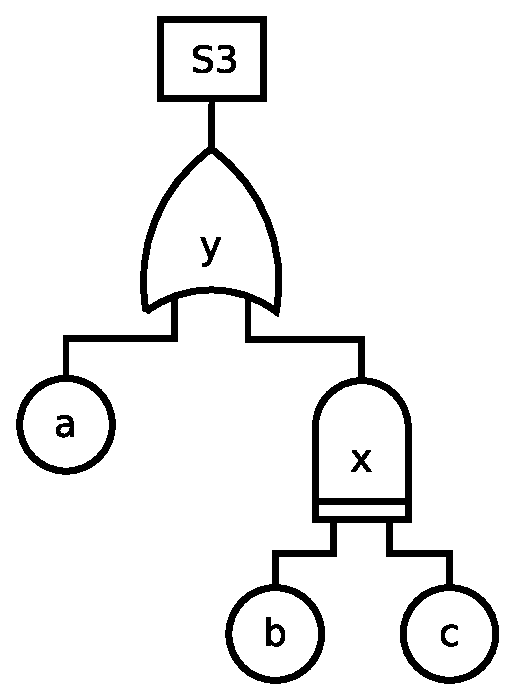
\includegraphics[height=4.0cm]{s3}
  \caption{Пример дерева отказов с узлом PAND.}
  \label{fig:dft1}
\end{figure}

Однако, тут есть тонкий момент. Для примера рассмотрим дерево отказов, изображённое на рисунке \ref{fig:dft1}. Его общее распределение, согласно сказанному выше, будет иметь вид:

\begin{equation*}
  g_{abcxy} = \lambda_a e^{-\lambda_a t_a} \lambda_b e^{-\lambda_b t_b}
  \lambda_c e^{-\lambda_c t_c} \delta(t_x - t_c) \theta(t_c - t_b)
  [\delta(t_y - t_a) \theta(t_x - t_a) + \delta(t_y - t_x) \theta(t_a - t_x)].
\end{equation*}

Поскольку корнем этого дерева является узел OR, а первый потомок этого узла -- это элементарное событие $A$, то полный интеграл по всем переменным распределения должен быть равен $1$, так как событие $Y$ когда-нибудь гарантированно произойдёт. Проинтегрируем в следующем порядке: $Y$, $X$, $A$, $C$, $B$:

\begin{align*}
  \int\limits_0^{+\infty} g_{abcxy} \dif t_y &= \lambda_a e^{-\lambda_a t_a}
  \lambda_b e^{-\lambda_b t_b} \lambda_c e^{-\lambda_c t_c}
  \delta(t_x - t_c) \theta(t_c - t_b) [\theta(t_x - t_a) + \theta(t_a - t_x)] = \\
  &= \lambda_a e^{-\lambda_a t_a} \lambda_b e^{-\lambda_b t_b}
  \lambda_c e^{-\lambda_c t_c} \delta(t_x - t_c) \theta(t_c - t_b) = g_{abcx},
\end{align*}

\begin{equation*}
  \int\limits_0^{+\infty} g_{abcx} \dif t_x = \lambda_a e^{-\lambda_a t_a}
  \lambda_b e^{-\lambda_b t_b} \lambda_c e^{-\lambda_c t_c} \theta(t_c - t_b) = g_{abc},
\end{equation*}

\begin{equation*}
  \int\limits_0^{+\infty} g_{abc} \dif t_a =
  \lambda_b e^{-\lambda_b t_b} \lambda_c e^{-\lambda_c t_c} \theta(t_c - t_b) = g_{bc},
\end{equation*}

\begin{equation*}
  \int\limits_0^{+\infty} g_{bc} \dif t_c =
  \int\limits_{t_b}^{+\infty} \lambda_b e^{-\lambda_b t_b} \lambda_c e^{-\lambda_c t_c} \dif t_c
  = \lambda_b e^{-(\lambda_b + \lambda_c) t_b} = g_b,
\end{equation*}

\begin{equation*}
  \int\limits_0^{+\infty} g_b \dif t_b = \cfrac{\lambda_b}{\lambda_b + \lambda_c} \neq 1.
\end{equation*}

Как видно, полный интеграл по всем временам событий не получается равен $1$. Ошибка состоит в том, что распределения узлов AND (\ref{eq:andDistr}) и OR (\ref{eq:orDistr}) накладывают на распределения входящих в них событий $A$ и $B$ достаточно жёсткие требования, которым не удовлетворяет распределение PAND (\ref{eq:pandDistr1}). А именно, если посмотреть внимательно на доказательство (\ref{eq:andProve}), станет очевидно, что это доказательство предполагает равенство нулю вероятностей событий $A$ и $B$ в начальный момент времени ($G_a(0) = 0$ и $G_b(0) = 0$).

Аналогичная ситуация с OR. Доказательство (\ref{eq:orProve}) предполагает, что события $A$ и $B$ гарантированно когда-нибудь произойдут ($G_a(+\infty) = 1$ и $G_b(+\infty) = 1$). Однако именно этому условию и не удовлетворяет событие $X$ из дерева отказов на рисунке \ref{fig:dft1}, поскольку оно получено с помощью PAND и обладает шансом не реализоваться (то есть $G_x(+\infty) < 1$).

В принципе, то, что доказательства накладывают указанные ограничения, не показывает то, что сами формулы обладают этими ограничениями. Поэтому можно предположить, что доказательства недостаточно хороши, а сами формулы позволяют оперировать с распределениями, которые в нуле не равны нулю, а в бесконечности не приходят к единице. Однако, легко показать, что это не так. Например, если взять два события $A$ и $B$, одно из которых не происходит никогда $G_a(t) = 0$, то композиция двух эти событий с помощью узла OR должна давать просто распределение второго события $G(t) = G_b(t)$. Вместо этого получается $G(t) = 0$, что и показывает, что обсуждаемые ограничения наложены самими формулами для узлов AND и OR.

\subsubsection{Композиция PAND и OR}

Как было показано, нельзя использовать узел PAND в наивном изложении (\ref{eq:pandDistr1}), поскольку он создаёт распределение, которое на бесконечности не подходит к единице. Однако, в исследуемом формализме можно выразить композицию PAND и OR. То есть выразить распределение, у которого три потомка: в PAND заходят два из них, а в OR заходит результат PAND и третий. Распределение плотности вероятности выглядит следующим образом:

\begin{equation}
  \label{eq:pandOrDistr}
  g_{x|abc} = [\delta(t_x - t_b) \theta(t_c - t_b) + \delta(t_x - t_c) \theta(t_b - t_c)] \theta(t_b - t_a) + \delta(t_x - t_c) \theta(t_a - t_b).
\end{equation}

Такое распределение даёт на выходе распределение со всеми необходимыми свойствами(нуль в нуле и единица в бесконечности). Что легко показать:

\begin{equation}
  \label{eq:pandOrProve}
  \int\limits_0^{+\infty} g_{x|abc} \dif t_x
  = [\theta(t_c - t_b) + \theta(t_b - t_c)] \theta(t_b - t_a) + \theta(t_a - t_b)
  = \theta(t_b - t_a) + \theta(t_a - t_b) = 1.
\end{equation}

То, что указанное условное распределение семантически совпадает с тем, что должно быть, можно показать так же, как раньше, рассматривая разные порядки событий:

\begin{equation*}
  g_{x|abc} = \left\{
    \begin{array}{l}
      \delta(t_x - t_b) : t_a \leq t_b \leq t_c \\
      \delta(t_x - t_c) : t_b < t_a \cup t_c < t_b
    \end{array}
  \right. .
\end{equation*}

\section{Реализация}

Общее распределение строится из произведения экспоненциальных распределений базовых событий и условных распределений, состоящих из ступенчатых и дельта-функций. Для получения распределения по корневому событию общее распределение интегрируется по всем остальным событиям. При интегрировании суммы произведений ступенчатых функций, дельта-функций и экспонент получаются снова ступенчатые функции, дельта-фукнции и экспоненты. Причём технически процесс этого интегрирования достаточно прост, что наводит на мысль об автоматизации этого процесса. Поэтому текущий раздел посвящён алгоритмизации аналитического интегрирование общего распределения.

\subsection{Структура подынтегрального выражения}

Под интегралом стоит некоторое выражение, которое после раскрытия всех скобок и приведения подобных слагаемых становится суммой элементарных слагаемых(называемых далее ``атомарными''). Например, рассмотрим простое дерево отказов, изображённое на рисунке \ref{fig:dft1}. В совместную плотность распределения этого дерева входят четыре множителя:

\begin{equation*}
  \begin{array}{l}
    \lambda_a e^{-\lambda_a t_a}, \\
    \lambda_b e^{-\lambda_b t_b}, \\
    \lambda_c e^{-\lambda_c t_c}, \\
    \left[\delta(t_x - t_b) \theta(t_c - t_b) + \delta(t_x - t_c) \theta(t_b - t_c)\right]
    \theta(t_b - t_a) + \delta(t_x - t_c) \theta(t_a - t_b).
  \end{array}
\end{equation*}

Чтобы получить плотность распределения корневого события(которая зависит только от $t_x$), нужно проинтегрировать от $0$ до $+\infty$ по остальным переменным, а именно по $t_a$, $t_b$, $t_c$. Пусть первой переменной в очереди на интегрирование будет $t_a$. Чтобы по ней проинтегрировать, нужно взять интеграл по произведению от первого и четвёртого множителей, поскольку только они зависят от $t_a$. Интеграл будет выглядеть следующим образом:

\begin{equation*}
  \int\limits_0^{+\infty}
  \left(
    \left[
      \delta(t_x - t_b) \theta(t_c - t_b) + \delta(t_x - t_c) \theta(t_b - t_c)
    \right]
    \theta(t_b - t_a) + \delta(t_x - t_c) \theta(t_a - t_b)
  \right)
  \lambda_a e^{-\lambda_a t_a} \dif t_a.
\end{equation*}

После раскрытия скобок получаем:
\begin{align*}
  \int\limits_0^{+\infty}
  [
    & \delta(t_x - t_b) \theta(t_c - t_b) \theta(t_b - t_a) \lambda_a e^{-\lambda_a t_a} + \\
    & + \delta(t_x - t_c) \theta(t_b - t_c) \theta(t_b - t_a) \lambda_a e^{-\lambda_a t_a} + \\
    & + \delta(t_x - t_c) \theta(t_a - t_b) \lambda_a e^{-\lambda_a t_a}
  ] \dif t_a.
\end{align*}

Как видно, под интегралом стоит сумма из слагаемых специально вида, а именно это одночлены, состоящие из:
\begin{itemize}
\item константы (в данном случае она всюду равна $\lambda_a$),
\item произведения дельта-функций от разности двух переменных,
\item произведения ступенчатых функций от разности двух переменных,
\item экспоненты.
\end{itemize}
Именно такого вида одночлены мы и будем называть ``атомарными''. Дальнейшее изложение раздела заключается в том, чтобы выстроить алгоритм интегрирования атомарного одночлена. Этого вполне достаточно, поскольку любое получаемое в дальнейшем выражение будет раскладываться в эти атомарные слагаемые, а интеграл от суммы атомарных слагаемых -- это сумма интегралов от этих самых слагаемых.

\subsection{Интегрирование ``дельтой''}

Рассмотрим сначала, что делать с дельта-функциями в атомарном одночлене при интегрировании по переменной $t$. Во-первых, дельта-функции, в которых нет $t$, в интегрировании не участвуют, а просто выносятся за знак интеграла. Во-вторых, когда под дельта-функцией $t$ присутствует, тогда значение всего интеграла определяется этой дельта-функцией. Проще говоря:

\begin{equation}
  \label{eq:int1}
  \int_{\alpha}^{\beta} \delta(t - \gamma) F(t) \dif t
  = \theta(\beta - \gamma) \theta(\gamma - \alpha) F(\gamma).
\end{equation}

$F(t)$ -- некоторая функция, в которой сосредоточена вся остальная часть интегрируемого атомарного одночлена. Тут показано, что при интегрировании ``дельтой'' $t$ во всём оставшемся выражении заменяется на $\gamma$ согласно определению дельта-функции, данному ранее.

В том случае, когда под интегралом стоит $\delta(\gamma - t)$, а не рассмотренное $\delta(t - \gamma)$, интегрирование происходит точно так же. Это корректно благодаря чётности дельта-функции.

О множителях $\theta(\beta - \gamma) \theta(\gamma - \alpha)$ следует сказать особо. Они учитывают факт того, что $\gamma$ может не лежать внутри пределов интеграла. То есть, если вдруг окажется, что $\gamma > \beta$, тогда результат интегрирования занулится. В итоговом выражении за это отвечает можитель $\theta(\beta - \gamma)$. В противном случае $\gamma < \beta$ умножение на единицу не сыграет роли.

Когда верхним пределом интеграла является $+\infty$, множитель $\theta(\beta - \gamma)$ пропадает, поскольку условие $\gamma < +\infty$ выполняется всегда.

\subsection{Интегрирование ``ступенькой''}

Когда среди дельта-функций в атомарном одночлене нет переменной, по которой ведётся интегрирование, можно переходить к рассмотрению ступенчатых функций. Ступенчатая функция не является чётной, поэтому придётся рассматривать два варианта: $\theta(t - \gamma)$ и $\theta(\gamma - t)$.

\subsubsection{Положительная ступенька}

Под положительной ступенькой подразумевается присутствие множителя $\theta(t - \gamma)$ в подынтегральном выражении при интегрировании по $t$. В таком случае интеграл раскрывается следующим образом:

\begin{equation}
  \label{eq:int2}
  \int\limits_{\alpha}^{\beta} \theta(t - \gamma) F(t) \dif t
  = \theta(\beta - \gamma) \theta(\gamma - \alpha) \int\limits_{\gamma}^{\beta} F(t) \dif t
  + \theta(\alpha - \gamma) \int\limits_{\alpha}^{\beta} F(t) \dif t.
\end{equation}

Во-первых, чтобы обосновать эту формулу, просто рассмотрим различные варианты расположения границ интегрировани ($\alpha$ и $\beta$) и начала ступеньки:

\begin{equation*}
  \int\limits_{\alpha}^{\beta} \theta(t - \gamma) F(t) \dif t
  = \left\{
    \begin{array}{ll}
      \int\limits_{\alpha}^{\beta} F(t) \dif t, &\gamma \leq \alpha \\
      \int\limits_{\gamma}^{\beta} F(t) \dif t, &\alpha < \gamma \leq \beta \\
      0, &\beta < \gamma
    \end{array}
  \right. .
\end{equation*}

Во-вторых, следует отметить, что указанная формула опирается на тот факт, что $\alpha \leq \beta$, чтобы не порождать множество бесполезных условий в виде $\theta(\alpha - \beta)$, которые потом придётся интегрировать. В силу этого, нужно чётко соблюдать факт того, что нижний предел интегрирования должен быть меньше верхнего предела.

В-третьих, отдельно следует рассмотривать случай, когда верхней границей является бесконечность:

\begin{equation}
  \label{eq:int3}
  \int\limits_{\alpha}^{+\infty} \theta(t - \gamma) F(t) \dif t
  = \theta(\gamma - \alpha) \int\limits_{\gamma}^{+\infty} F(t) \dif t
  + \theta(\alpha - \gamma) \int\limits_{\alpha}^{+\infty} F(t) \dif t.
\end{equation}

\subsubsection{Отрицательная ступенька}

Аналогично, под отрицательной ступенькой подразумевается присутствие множителя $\theta(\gamma - t)$ в подынтегральном выражении при интегрировании по $t$. Раскрывается следующим образом:

\begin{equation}
  \label{eq:int4}
  \int\limits_{\alpha}^{\beta} \theta(\gamma - t) F(t) \dif t
  = \theta(\beta - \gamma) \theta(\gamma - \alpha) \int\limits_{\alpha}^{\gamma} F(t) \dif t
  + \theta(\gamma - \beta) \int\limits_{\alpha}^{\beta} F(t) \dif t.
\end{equation}

Корректность формулы демонстрируется так же, как и раньше:

\begin{equation*}
  \int\limits_{\alpha}^{\beta} \theta(\gamma - t) F(t) \dif t
  = \left\{
    \begin{array}{ll}
      0, &\gamma \leq \alpha \\
      \int\limits_{\alpha}^{\gamma} F(t) \dif t, &\alpha < \gamma \leq \beta \\
      \int\limits_{\alpha}^{\beta} F(t) \dif t, &\beta < \gamma
    \end{array}
  \right. .
\end{equation*}

И ещё так же, как и раньше, отдельно рассматривается случай бесконечной верхней границы интегрирования:

\begin{equation}
  \label{eq:int5}
  \int\limits_{\alpha}^{+\infty} \theta(\gamma - t) F(t) \dif t
  = \theta(\gamma - \alpha) \int\limits_{\alpha}^{\gamma} F(t) \dif t.
\end{equation}

\subsection{Интегрирование ``экспонентой''}

В том случае, когда не осталось ни дельта-функций с интегрируемой переменной, ни ступенек, у атомарного одночлена остаётся лишь экспоненциальная часть, которая интегрируется очевидным образом:

\begin{equation}
  \label{eq:int6}
  \int\limits_{\alpha}^{\beta} e^{-\lambda t} \dif t = \cfrac{1}{\lambda}\left(e^{-\lambda \alpha} - e^{-\lambda \beta}\right).
\end{equation}

\subsection{Итого}

Подводя итог. В том случае, когда под интегралом есть дельта-функции, содержащие переменную интегрирования, интегрирование производится по формуле \ref{eq:int1}. Когда дельта-функций, содержащих переменную интегрирования, нет, но есть ступеньки с этой переменной, интегрирование проводится по формулам \ref{eq:int2}, \ref{eq:int3}, \ref{eq:int4} и \ref{eq:int5}. Когда ни в дельта-функциях, ни в ступеньках нет переменной интегрирования, остаётся лишь экспонента, которая интегрируется тривиально (см. \ref{eq:int6}).

\begin{thebibliography}{9}

\bibitem{barel}
  Boundali, Dougan.
  \emph{A Continuous-Time Bayesian Network Reliability Modeling, and Analysis Framework}.
  IEEE Transactions on Reliability,
  2006.

\end{thebibliography}

\end{document}
%%% Local Variables: 
%%% mode: latex
%%% TeX-master: t
%%% End: 
